\chapter{Interfacing With The Kinect Sensor}
\ifpdf
    \graphicspath{{Chapter3/Chapter3Figs/PNG/}{Chapter3/Chapter3Figs/PDF/}{Chapter3/Chapter3Figs/}}
\else
    \graphicspath{{Chapter3/Chapter3Figs/EPS/}{Chapter3/Chapter3Figs/}}
\fi

% ------------------------------------------------------------------------

The Kinect SDK provides access to the Kinect Sensor from within C\# code by defining a \verb|KinectSensor| object which interfaces directly with the hardware. When this object is instantiated, and provided a Kinect Sensor is connected via the USB port, it provides access to the depth, RGB and skeletal streams of the camera. The \verb|KinectSensor| object also contains an event  \verb|AllFramesReady| which fires each time the streams have successfully updated. The streams update at approximately 30 frames per second but this rate can be significantly reduced if the sensor attempts to track too many skeletons. Using this \verb|KinectSensor| object we built a general purpose skeletal tracking controller class \verb|GestureController| (Figure: ~\ref{fig:umlgest}) which initialises a \verb|KinectSensor| object to provide a single skeletal stream (for the left most person in the camera shot) and subscribes to the \verb|AllFramesReady| event via the method \verb|KinectAllFramesReady|.

\section{Recording Training Data}
In order to record the training data we implemented a class \verb|GestureRecorder|, which extends \verb|GestureController|, and a class \verb|GestureRecording| which stores a single recording of the skeleton over time(Figure: ~\ref{fig:umlgest}). This second class contains a hashmap from \verb|JointType| (an enum listing the different possible joints tracked by the Kinect Sensor) to a list of 3-vectors representing the readings of that joint through time, and a method \verb|addReading| which takes a \verb|Skeleton| object and adds each joint location to the appropriate list. The \verb|GestureRecorder| class stores a list of completed \verb|GestureRecording| objects, along with one which is the current recording, and extends the \verb|KinectAllFramesReady| method to pass the Skeleton provided by the sensor to the \verb|currentRecording| object. This class also provides methods to start and stop the current recording (adding it to the list of recordings when stopped) and to save the list of recordings to file. This \verb|GestureRecorder| class allows us to record the movements of the hands, wrists, elbows, shoulders and head over time and save them as training data. Further we implemented two methods for storing the data - as positions relative to the camera or as positions releative to the signer's head. This second method of storing positions prevents the same sign creating different readings when performed at different distances from the camera, in a different environment or by a different signer. It is these head relative distances that we use to train the sign models.


\begin{figure}[h!]
        \centering
        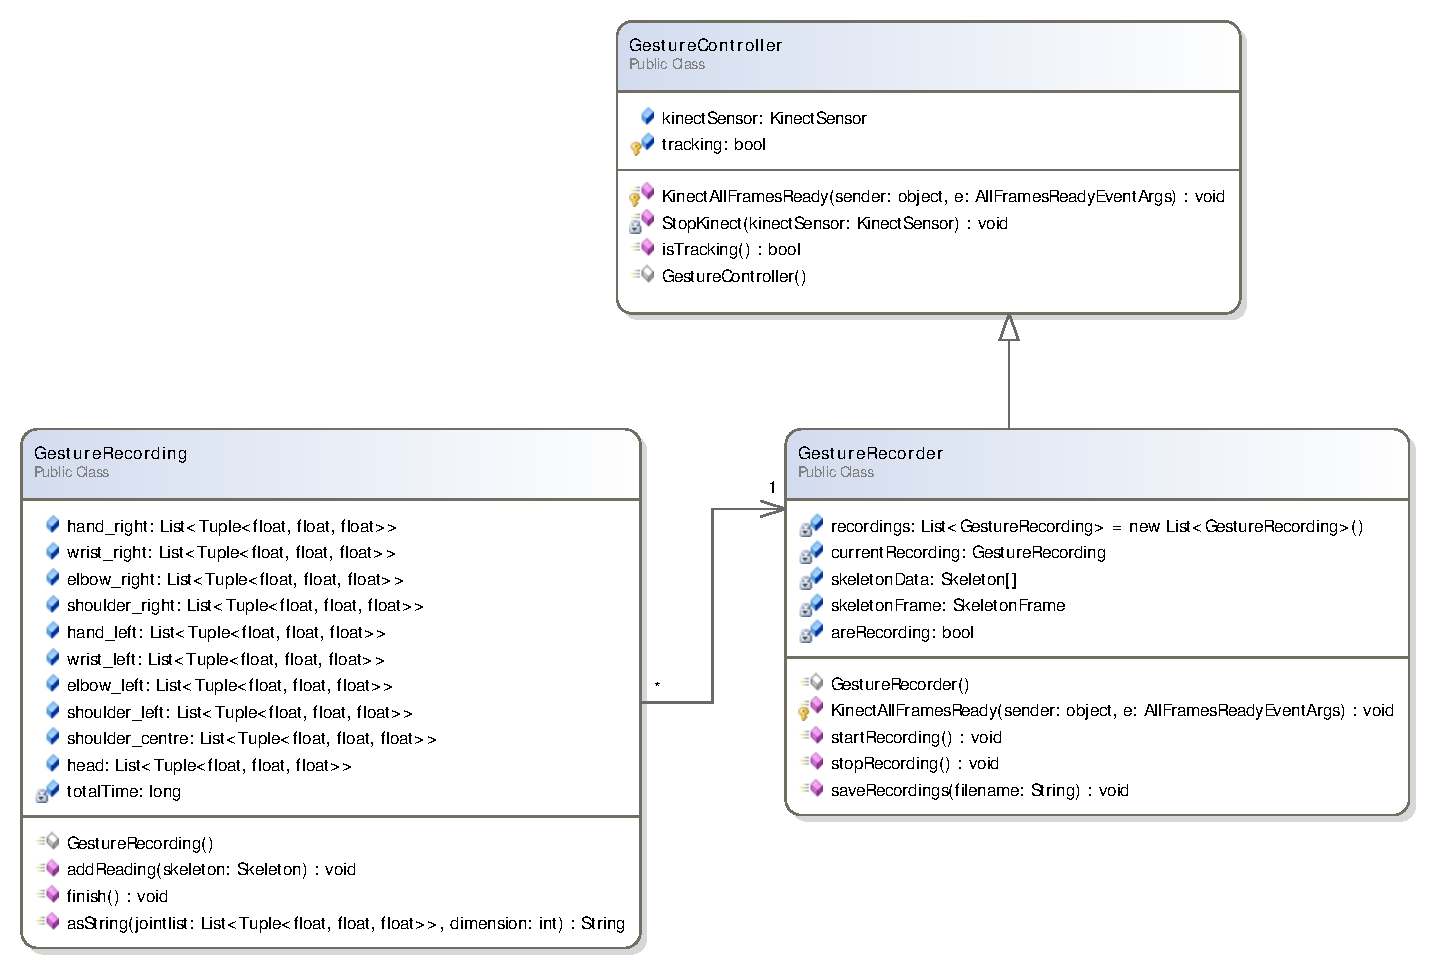
\includegraphics[width = 1.0\textwidth]{ThesisFigs/gestRecDiag}
        \caption{A UML diagram of the gesture recording classes}\label{fig:umlgest}
\end{figure}

Using this controller we implemented a small program which can be used to record a collection of training data by repeating the sign the desired number of times and giving a start/stop signal between each. For convenience we defined this signal to be when hands are raised a certain distance above the waist, a signal consistent with the pose a signer takes whilst pausing between sequences of signs.
 
\subsection{The Training Data}
Using this controller we recorded for each of a collection of 30 British Sign Language (See Figure:) signs a set of 40 training examples and a further set of 10 testing examples. Each sign lasted between 1 and 2 seconds and was recorded at the maximum skeletal frame rate - 30 frames per second.

\subsection{Limitations in the Training Data}
The quality of the training sets was degraded by two factors. The first is that the signer (myself) that performed the training sets is not fully fluent in sign language and hence does not reproduce the signs consistently, this introduced inconsistencies into the training set and caused it to contain instances of signs that a fluent signer might not ever make. The second factor is a  limitation of the Kinect Sensor. The Kinect can track joints well when they are isolated but performs poorly when two parts of the body, for example the hands, are in contact~\ref{fig:brokht} and as many common signs require the hands to be placed together this issue caused a significant amount of the noise in the training data for those signs. The hand tracking issue is expect to be fixed in an upcoming SDK release but the contact issue could still caused noise in certain signs, for example those that require the signer to touch their elbows, shoulders or face.

\begin{figure}[h!]
        \centering
        \includegraphics[width = 1.0\textwidth]{ThesisFigs/brokenHandTracking}
        \caption{An example of the broken hand tracking with the hands placed together. The yellow joints are inferred by the sensor incorrectly, the actual location of the hands is just below the chin.}\label{fig:brokht}
\end{figure}


%%% Local Variables: 
%%% mode: latex
%%% TeX-master: "../thesis"
%%% End: 
